% !TeX program = xelatex
% !TeX encoding = UTF-8
\documentclass[fontset=none,zihao=-4,a4paper]{ctexart}

\usepackage{geometry}
\usepackage{amsmath,amssymb}
\usepackage{graphicx,booktabs,array,longtable}
\usepackage{xcolor,listings,float}
\usepackage{enumitem,setspace,tocloft}
\usepackage{hyperref}
\geometry{left=2.5cm,right=2.5cm,top=2.5cm,bottom=2.5cm}

% 中文宋体/黑体；英文及数字使用 Times New Roman。
\setmainfont{Times New Roman}
\setsansfont{Times New Roman}
\setmonofont{Times New Roman}
\setCJKmainfont[AutoFakeBold=2.5]{SimSun}
\setCJKsansfont[AutoFakeBold=2.5]{SimHei}
\setCJKmonofont[AutoFakeBold=2.5]{SimSun}
\setCJKfamilyfont{zhsong}[AutoFakeBold=2.5]{SimSun}
\setCJKfamilyfont{zhhei}[AutoFakeBold=2.5]{SimHei}
\newcommand{\songti}{\CJKfamily{zhsong}}
\newcommand{\heiti}{\CJKfamily{zhhei}}

% 正文宋体小四，1.25倍行距，段前段后0，首行缩进两个汉字。
\setstretch{1.25}
\setlength{\parskip}{0pt}
\AtBeginDocument{\songti\zihao{-4}\setlength{\parindent}{2\ccwd}}
\raggedbottom
\pagestyle{plain}
\ctexset{
  section={format={\raggedright\heiti\zihao{4}\bfseries},
    beforeskip=0pt,afterskip=0pt,afterindent=true},
  subsection={format={\raggedright\heiti\zihao{4}\mdseries},
    beforeskip=0pt,afterskip=0pt,afterindent=true},
  subsubsection={format={\raggedright\songti\zihao{4}\mdseries},
    beforeskip=0pt,afterskip=0pt,afterindent=true}
}
\setcounter{secnumdepth}{3}
\setcounter{tocdepth}{3}
\setlist{topsep=0pt,partopsep=0pt,parsep=0pt,itemsep=0pt}

\renewcommand{\cfttoctitlefont}{\heiti\zihao{4}\bfseries}
\setlength{\cftbeforetoctitleskip}{0pt}
\setlength{\cftaftertoctitleskip}{0pt}
\setlength{\cftbeforesecskip}{0pt}
\setlength{\cftbeforesubsecskip}{0pt}
\setlength{\cftbeforesubsubsecskip}{0pt}
\renewcommand{\cftsecfont}{\songti\zihao{-4}\mdseries}
\renewcommand{\cftsecpagefont}{\rmfamily\zihao{-4}\mdseries}
\renewcommand{\cftsubsecfont}{\songti\zihao{-4}\mdseries}
\renewcommand{\cftsubsecpagefont}{\rmfamily\zihao{-4}\mdseries}
\renewcommand{\cftsubsubsecfont}{\songti\zihao{-4}\mdseries}
\renewcommand{\cftsubsubsecpagefont}{\rmfamily\zihao{-4}\mdseries}

\lstset{
  basicstyle=\ttfamily\songti\zihao{-4},
  keywordstyle=\color{blue},commentstyle=\color{gray},
  stringstyle=\color{red!70!black},
  numbers=left,numberstyle=\rmfamily\scriptsize\color{gray},
  stepnumber=1,numbersep=8pt,frame=single,
  breaklines=true,showstringspaces=false,keepspaces=true,
  tabsize=4,columns=fullflexible,
  aboveskip=0.5\baselineskip,belowskip=0.5\baselineskip,
  escapeinside={(*@}{@*)}
}
\hypersetup{colorlinks=true,linkcolor=black,urlcolor=blue,citecolor=black}

\begin{document}
{\centering\heiti\zihao{3}\bfseries
实验一：NLP前置技术——Python环境搭建\par}
\tableofcontents
\newpage

\section{实验目的}
	
	本实验主要完成自然语言处理课程所需 Python 环境的搭建，并熟悉常用 NLP 工具的基本使用方法。通过本次实验，需要掌握 Python 运行环境及相关依赖库的配置方法，学会使用 Jupyter Notebook 进行代码编写和运行，并完成简单的中文和英文文本处理任务。
	
	具体实验目标如下：
	
	\begin{enumerate}
		\item 掌握 Python 及 Anaconda 环境的基本使用方法；
		\item 掌握常用 Python 第三方库的安装与管理方法；
		\item 熟悉 Jupyter Notebook 的基本操作；
		\item 掌握 jieba 中文分词工具的基本使用方法；
		\item 掌握 NLTK 英文分词工具的基本使用方法；
		\item 使用 Counter 对分词结果进行简单的词频统计；
		\item 学会分析并解决 Python 环境配置和资源缺失等常见问题。
	\end{enumerate}
	
	% ==================================================
	\section{实验环境}
本次实验使用Anaconda提供的Python环境，在Jupyter Notebook中编写和运行程序。主要依赖包括NumPy、pandas、Matplotlib、scikit-learn、jieba和NLTK。

实验开始后，通过导入相关库并打印版本信息，对当前环境进行验证。代码和实际输出见图\ref{fig:environment}。

\begin{figure}[H]
\centering
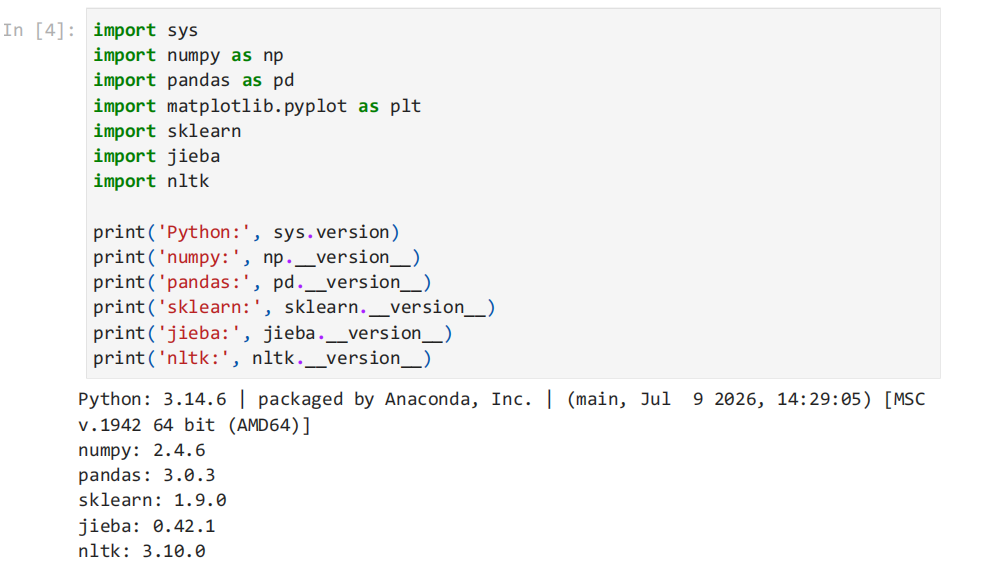
\includegraphics[width=\linewidth]{NLP_exp1_images/environment.png}
\caption{Python环境与相关库的实际版本检查}\label{fig:environment}
\end{figure}

截图中的Python版本为3.14.6，jieba版本为0.42.1，NLTK版本为3.10.0，相关库均已成功导入。教师Notebook中的环境创建示例使用Python 3.10，本报告记录的实际版本以图中输出为准。

\section{实验内容与步骤}
	
	\subsection{Python环境及依赖库配置}
	
	首先检查 Python 和 Conda 环境是否已经正确安装，可以在命令行中输入：
	
	\par\noindent\begin{minipage}[t]{\linewidth}
\begin{lstlisting}[language=bash, caption={Python与Conda版本检查}]
python --version
conda --version
	\end{lstlisting}
\end{minipage}\par
	
	根据实验要求，可以通过 pip 安装自然语言处理所需的常用 Python 库，例如：
	
	\par\noindent\begin{minipage}[t]{\linewidth}
\begin{lstlisting}[language=bash, caption={相关依赖库安装}]
pip install numpy pandas matplotlib scikit-learn jieba nltk jupyter ipykernel
	\end{lstlisting}
\end{minipage}\par
	
	安装完成后，可以使用如下命令查看当前环境中已经安装的 Python 软件包：
	
	\par\noindent\begin{minipage}[t]{\linewidth}
\begin{lstlisting}[language=bash]
pip list
	\end{lstlisting}
\end{minipage}\par
	
	通过上述步骤，为后续中文分词、英文分词以及其他自然语言处理实验建立基础运行环境。
	
	\subsection{Jupyter Notebook环境配置}
	
	完成 Python 及相关第三方库的安装后，本实验使用 Jupyter Notebook 作为开发环境。
	
	为了保证 Jupyter Notebook 使用正确的 Python 环境，可以将当前环境注册为 Jupyter 内核：
	
	\par\noindent\begin{minipage}[t]{\linewidth}
\begin{lstlisting}[language=bash, caption={Jupyter内核注册}]
python -m ipykernel install --user --name nlp --display-name "Python (NLP)"
	\end{lstlisting}
\end{minipage}\par
	
	之后可以通过以下命令启动 Jupyter Notebook：
	
	\par\noindent\begin{minipage}[t]{\linewidth}
\begin{lstlisting}[language=bash]
jupyter notebook
	\end{lstlisting}
\end{minipage}\par
	
	启动完成后，浏览器会自动进入 Notebook 页面，即可进行代码编写与运行。
	
	% ==================================================
	\section{中文分词与词频统计实验}
\subsection{代码与运行结果}
本实验使用jieba对给定中文文本进行分词，再使用Counter统计分词列表中各词元的出现次数。代码、分词结果和前10项词频见图\ref{fig:chinese}。

\begin{figure}[H]
\centering
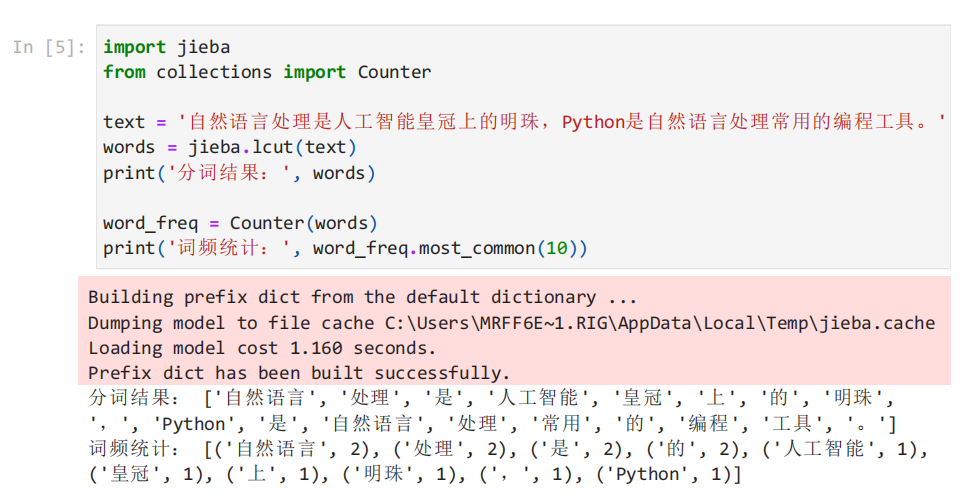
\includegraphics[width=\linewidth]{NLP_exp1_images/chinese_segmentation.png}
\caption{jieba中文分词与词频统计的运行结果}\label{fig:chinese}
\end{figure}

\subsection{结果说明}
分词结果中，“自然语言”和“处理”被划分为独立词元，中英混合文本中的Python也被保留。“自然语言”“处理”“是”“的”均出现2次，与原句中的重复情况一致。逗号和句号同样出现在分词列表中，且逗号进入了前10项词频结果，说明程序尚未进行标点过滤。

\section{英文分词实验}
\subsection{代码与运行结果}
本实验使用NLTK提供的\texttt{word\_tokenize()}对给定英文句子进行分词。程序和实际输出见图\ref{fig:english}。

\begin{figure}[H]
\centering
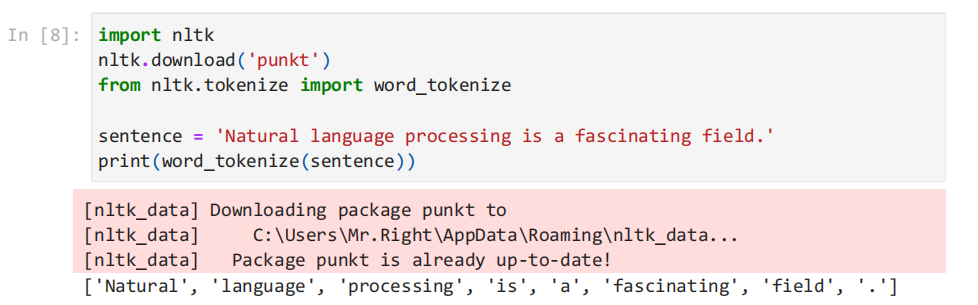
\includegraphics[width=\linewidth]{NLP_exp1_images/english_tokenization.png}
\caption{NLTK英文分词的运行结果}\label{fig:english}
\end{figure}

\subsection{结果说明}
程序将英文句子划分为7个单词和一个句点，句点作为独立词元保留。截图中的资源提示表明punkt已存在且处于最新状态，随后分词程序正常输出词元列表。

\section{实验中遇到的问题及解决方法}
\subsection{jieba模块缺失与安装检查}
初次导入jieba时，程序提示当前环境无法找到该模块。处理这一问题时，需要保证jieba安装在Jupyter Notebook实际使用的Python环境中，而不是其他环境。

实验中保留的安装命令如图\ref{fig:jieba-install}所示。

\begin{figure}[H]
\centering
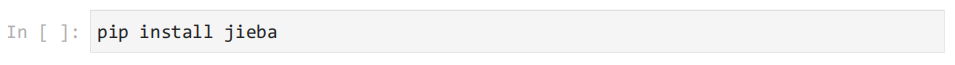
\includegraphics[width=\linewidth]{NLP_exp1_images/jieba_install.png}
\caption{jieba安装命令记录}\label{fig:jieba-install}
\end{figure}

这张截图的单元格执行编号为空，未展示安装输出，因此仅作为安装命令记录。后续图\ref{fig:environment}显示jieba能够成功导入，图\ref{fig:chinese}也保存了正常分词结果，可以据此确认后续运行时该模块已可用。

\subsection{NLTK数据资源缺失}
在进行英文分词时，遇到了punkt\_tab资源无法找到的提示。NLTK软件包能够导入，并不代表分词所需的数据资源已经齐全，因此需要另行检查和补充资源。

资源下载过程见图\ref{fig:nltk-resources}。

\begin{figure}[H]
\centering
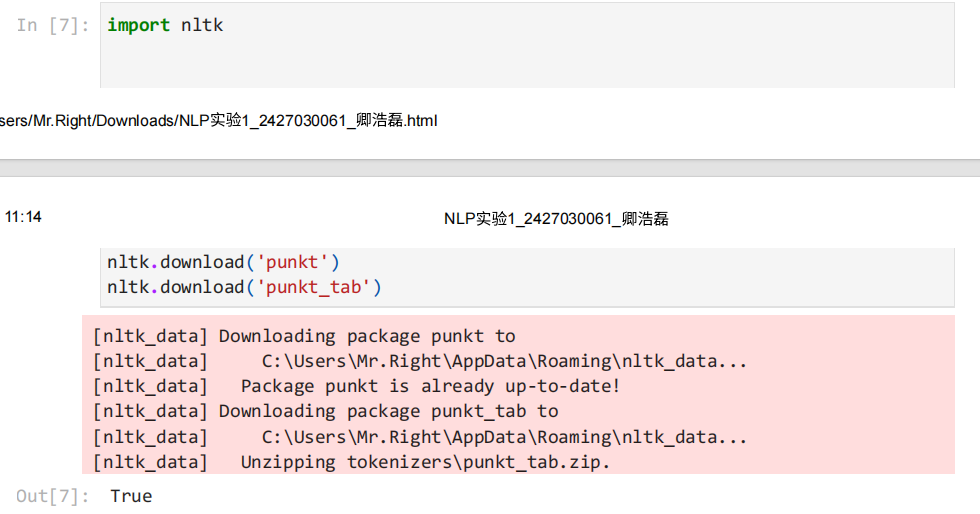
\includegraphics[width=\linewidth]{NLP_exp1_images/nltk_resources.png}
\caption{NLTK分词资源检查与punkt\_tab下载记录}\label{fig:nltk-resources}
\end{figure}

记录显示punkt已存在，punkt\_tab被下载并解压，单元格返回True。补充资源后，英文分词程序正常输出结果，如图\ref{fig:english}所示。该过程说明，环境验证应同时检查Python依赖库和具体任务所需的数据资源。

\section{实验结果分析}
	
	通过本次实验可以发现，中文和英文文本在分词方式上存在明显区别。
	
	英文单词之间通常存在空格，因此可以较容易地根据空格和标点识别单词边界。例如：
	
	\par\noindent Natural language processing\par
	
	可以自然划分为：
	
	\par\noindent Natural\\
language\\
processing\par
	
	而中文文本通常连续书写，词语之间没有天然空格。例如：
	
	\par\noindent 自然语言处理是人工智能的重要技术\par
	无法直接根据字符之间的位置判断词语边界，因此需要借助 jieba 等中文分词工具，根据词典及概率模型对句子进行合理切分。
	
	此外，从实验结果中还可以看出，无论是 jieba 还是 NLTK，都可能将标点符号作为 token 保留下来。在实际文本分析或机器学习任务中，通常还需要进行数据清洗，例如删除标点符号、停用词以及无意义字符。
	
	因此，自然语言处理中的文本预处理往往不仅包含分词，还包括文本清洗、标准化以及停用词去除等步骤。
	
	% ==================================================
	\section{思考与分析}
	
	\subsection{为什么中文不能简单使用空格进行分词？}
	
	英文单词之间通常存在天然空格，可以较容易地按照空格进行切分，而中文句子中的词语通常连续书写，不存在明显的词语边界。
	
	例如：
	
	\par\noindent 自然语言处理技术\par
	
	可以理解为：
	
	\par\noindent 自然语言 / 处理 / 技术\par
	
	因此，需要借助中文分词算法，根据词典、统计概率或者语言模型判断词语边界。
	
	\subsection{为什么标点符号会出现在分词结果中？}
	
	分词程序通常将文本按照字符和词语边界进行切分，并不会自动认定标点符号没有意义，因此中文逗号、句号，以及英文句点等符号都有可能作为独立 token 被保留下来。
	
	是否删除这些标点符号，需要根据具体自然语言处理任务决定。
	
	\subsection{如何删除标点符号？}
	
	可以在分词完成后对结果进行筛选，例如：
	
	\par\noindent\begin{minipage}[t]{\linewidth}
\begin{lstlisting}[language=Python]
words = [
word for word in words
if word.strip() and word not in '，。！？；：、“”‘’'
]
	\end{lstlisting}
\end{minipage}\par
	
	也可以使用正则表达式实现更加全面的文本清洗。
	
	% ==================================================
	\section{实验总结}
通过本次实验，我熟悉了Anaconda环境中Python依赖库的检查方法和Jupyter Notebook的基本操作，并完成了jieba中文分词、NLTK英文分词及Counter词频统计。

实验中检查了jieba与当前运行环境的对应关系，并补充下载了英文分词所需的资源。环境验证、中文分词和英文分词的截图保存了实际代码及输出，可用于检查依赖与资源是否可用。

从结果中可以看出，中文和英文的词语边界处理方式不同，分词也不会自动完成标点过滤。词频统计反映词元在给定文本中的出现次数，结果的解释需要结合原始文本和是否进行清洗来判断。

\end{document}